\documentclass[a4paper]{article}
\usepackage{amsmath}
%\usepackage[a4paper, total={15cm, 20cm}]{geometry}
\usepackage{graphicx}
\usepackage{hyperref}
\usepackage{indentfirst}
\hypersetup{colorlinks=true, linkcolor=blue}

%% Documents settings
\title{Projet d'optimisation}
\author{Vasavan \& Wesley}

\begin{document}
%% Generate the title
\maketitle
\newpage
\protect\hypertarget{table}{}
\renewcommand{\contentsname}{Sommaire}
\tableofcontents
\newpage
\newpage

\section{Objectif}
La mission d'un lanceur spatial est d'amener un satellite en orbite. Le
 probl\`eme est divis\'e en deux parties l'impl\'ementation de l'algorithme SQP
 (Sequential Quadratic Programming) et l'impl\'ementation d'un simulateur, le
 tout en \textit{Matlab}.
\newpage

\section{Algorithme et logiciel}
\subsection{Optimisateur SQP}
L'algorithme SQP permet de r\'esoudre des probl\`emes non lin\'eaires sous
 contraintes.

\begin{figure}[h!]
\centering
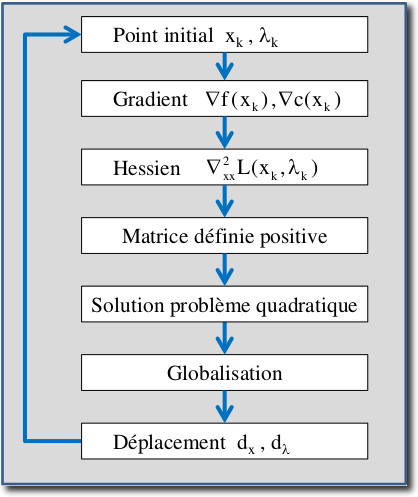
\includegraphics[width=6cm]{capture.png}
\caption{Organigramme}
\label{fig:1}
\end{figure}

\subsection{Calcul du gradient}
Le calcul du gradient est fait par diff\'erences finies.
\subsection{Calcul du hessien}
Le calcul du hessien est par une m\'ethode de Quasi-Newton. Les it\'erations
 sur la hessien sont faites soit par BFGS ou soit par SR1.
\subsection{Solution au probl\`eme quadratique}
\subsection{Globalisation}
\subsection{Test de l'algorithme}
Le premier test est MHW4D.

Les 10 premiers valeurs sont:

Les 10 derniers valeurs sont:

\section{Cas test: MHW4D}

\section{Lanceur}

\end{document}
